% Chapter 3

\chapter{Environment} % Main chapter title

\label{Chapter3} % For referencing the chapter elsewhere, use \ref{Chapter3} 

%----------------------------------------------------------------------------------------

In this chapter we report the process that went into choosing the environments that we will be using in the project's simulations, and from which we will be basing our simulations.

There are many choices of environments and tasks that are publicly available. Some of these we will be introducing in this chapter.

What makes this step non-trivial and deserving of its own chapter is that different reinforcement learning techniques are more suitable to different categories of tasks. Similarly, different machine learning and deep learning techniques are more or less efficient when applied to different tasks.

In a research effort that is heavily dependent on building reinforcement learning and deep learning models, the choice of environment is a critical one.

Furthermore, we also need to achieve this without losing focus on the main motivations for the whole project (Chapter~\ref{Chapter1}): \textit{optimising reinforcement learning algorithms by adding transferability of pre-trained models on unseen maps or configurations of a task}.

This last point implies that a substantial part of the computational work in the project will be about training hundreds of thousands of reinforcement learning models to build a dataset over a distribution of different maps (we present this in Chapter~\ref{Chapter4}). This is an important point: in the many experiments we ran, this turned out to be the biggest bottleneck, and required devices to distribute computations across multiple machines to make the computational time feasible in the timespan allocated to the project.

With these points in mind and given the experimental nature of the work, we conclude that a bottom-up approach in complexity is preferable. Given successful results with "easier" tasks, we can scale up in complexity and hopefully formalise and generalise our approach to more tasks (Chapter~\ref{Chapter7}).

Easier tasks will enable us to explore different reinforcement learning approaches that we introduced in Subsection~\ref{RL} with the guarantee that they will give satisfiable results. We can use these results as a foundation of the further steps (specifically Generative Adversarial Networks training in Chapter~\ref{Chapter5}).

Before introducing candidate environments, let us define what is meant by an "easy" reinforcement learning task. What we are looking for is ideally a task with a discrete and relatively small set of observable states and actions. Why does this condition make the task easier?

Imagine building a tree (such as the one shown in figure~\ref{fig:RLTree} with all possible states-action transitions, until we either: 1) reach a goal state, or 2) reach an arbitrarily maximum iteration time step $t = \eta$ or depth of the tree (to prevent infinite iterations). Also assume we were building this tree in a bruteforce manner (worst-case scenario of reinforcement learning resolutions), such that we need to build all possible paths or trajectory that the agent will need to take. Therefore, we would need to visit each node of the tree, until we arrive at the leaves, which will report the achieved reward for the agent given the path it has taken to get there.

The breath and depth of the state-action tree will increase as we increase the possible set of states we would need to traverse, adding up to the space and time complexity of our solution, which is exponential in $\#S$ and $\#A$ for both space and time ($\#S$ indicates the cardinality of a set S).

With that said, there is a solid line between our ideal environment and a trivial one that could be solved without the aid of reinforcement learning techniques.

Let's explore some candidate environments next.
\begin{figure}
\centering
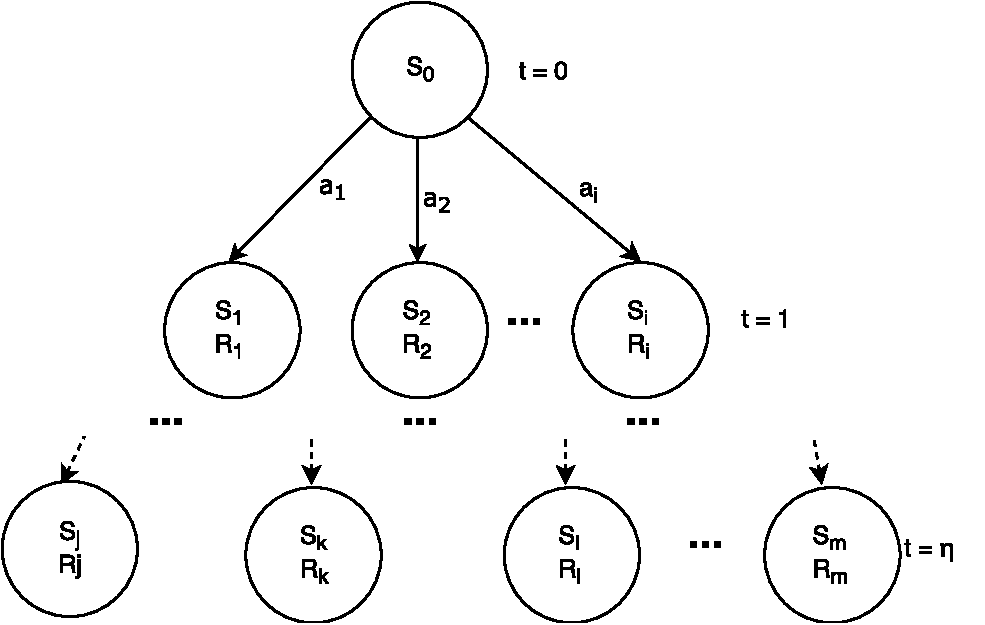
\includegraphics[width=7cm]{Figures/RLTree}
\caption{Sample state-action tree}
\label{fig:RLTree}
\end{figure}

\section{OpenAI Gym}
OpenAI Gym \citep{1606.01540} provides a toolkit that aids in the process of building reinforcement learning systems and evaluating algorithms to solve such tasks.

OpenAI Gym provides an environment interface \code{Env}. The interface abstracts the following operations on an environment:

\begin{itemize}
	\item \code{step(action)} -- Simulates one time step by executing the provided action. This returns \code{observation} (the new current state), the \code{reward} for taking such action, a flag \code{done} indicating whether the system has reached a final state, and \code{info} providing additional information dependent on the environment.
	\item \code{reset()} -- Resets the environment, i.e. the initial state is restored
	\item \code{render()} -- Renders the environment in human-readable format.
\end{itemize}

Now, we could either build implementations for such interface (if we were to implement our own environment's logic), or use the provided implementations for several environments in the OpenAI Gym library, which includes board games, algorithm-based or physics-based environments, Atari games, etc.

\subsection{Motivation}
In this project we will mostly deal with environments provided in the OpenAI Gym. There are several reasons for such decision:

\begin{itemize}
	\item it abstracts the need to implement the logic of a separate environment, adding a point of failure to our whole (quite experimental) work, as well as imposing a bigger time constraint to the one we already have;
	\item OpenAI Gym has become a standard academic tool for reinforcement learning researchers, therefore many papers and articles build on top of this framework;
	\item environment implementations are constantly expanding and being revised by an active community, also thanks to the support of the overarching organisation (OpenAI);
	\item the core implementation of the \code{gym} module allows for straightforward extensions on existing environments, which, as we will see in subsection~\ref{ExtendedBaseline}, will be critical in this project;
	\item while sadly not applicable anymore, OpenAI Gym used to provide and support an online platform for developers to compare the performance of different reinforcement learning algorithms for each task. This was in a form of a leaderboard, measuring the performance of the implementation, as well as providing the implementation and data of winning techniques. Such data could have been used directly as input to our Generative Adversarial Networks.
\end{itemize}

\subsection{Algorithmic environments}
\subsection{MuJoCo and physics environments}
\subsection{Other environments}

%----------------------------------------------------------------------------------------

\section{Baseline: \code{FrozenLake-v0}}
\subsection{Description of the task}
\subsection{Motivation}
\subsection{Shortcomings}

\section{Extended baseline: Randomised Frozen Lake}
\label{ExtendedBaseline}